\documentclass[mathserif,11pt]{beamer}

\usepackage{url,verbatim,natbib}
\usepackage[english]{babel}
\usepackage{amsmath, mathabx}
\usepackage{dsfont, ulem}
\usepackage{tikz}
\usepackage{xparse}
\newtheorem{proposition}[theorem]{Proposition}

\usepackage[headheight=22pt]{beamerthemeboxes}
\usepackage{graphicx}
\beamertemplatenavigationsymbolsempty 
\setbeamercovered{transparent}
\usepackage{centernot}

\setbeamertemplate{itemize item}{$\bullet$} 
\setbeamercolor{title}{fg=uio}
\setbeamertemplate{sections/subsections in toc}[ball unnumbered]
\setbeamercolor{section in toc}{fg=uio,bg=white}
\setbeamercolor{subsection in toc}{fg=uio,bg=white}
\setbeamercolor{result}{fg=black, bg=yellow}
\newcommand{\dotsim}{\stackrel{\cdot}{\sim}}
\newcommand{\interi}{{\rm Z}\negthinspace\negthinspace {\rm Z}}
\newcommand{\reali}{{\rm I}\negthinspace {\rm R}}
\newcommand{\naturali}{{\rm I}\negthinspace {\rm N}}
\newcommand{\sign}{\mathop{\rm sgn}\nolimits}
\newcommand{\sgn}{\mathop{\mathrm{sgn}}}
\definecolor{redve}{rgb}{0.604,0.008,0.00}
\definecolor{lmu}{rgb}{0.188,0.522,0.306}
\definecolor{uio}{rgb}{0.847,0.118,0.02}

\def\R{{\rm I\!R}}
\def\P{{\rm Pr}}
\def\Real{{\rm I\!R}}
\def\T{{\footnotesize {^{_{\sf T}}}}}
\def\tr{{\rm tr}}
\def\diag{{\rm diag}}

\NewDocumentCommand\DownArrow{O{2.0ex} O{black}}{%
   \mathrel{\tikz[baseline] \draw [<-, line width=0.5pt, #2] (0,0) -- ++(0,#1);}
}

\useframetitletemplate{% 
\begin{centering} 
\begin{small} \structure{\textcolor{uio} \insertframetitle {\insertframesubtitle}}
\end{small}

\end{centering} 
}

\addheadboxtemplate{\color[rgb]{1,1,1}}{\color{uio} \underline{{\hspace{5pt}\includegraphics[scale=0.06]{../../../../support/uio_logo_eng} \hspace{0.265\paperwidth}\color{black} \tiny  STK-IN4300 - Statistical Learning Methods in Data Science} \hspace{5pt}}}

%\bfseries{\insertsection}

\addfootboxtemplate{\color[rgb]{1,1,1}}{\color{black} \tiny \quad  
STK-IN4300: lecture 13
  \hfill \tiny \insertframenumber / \inserttotalframenumber \hspace{5pt}}

  
\title{STK-IN4300 \\ Statistical Learning Methods in Data Science}
\author{Riccardo De Bin} 
\institute{debin@math.uio.no} 
\date{}


\begin{document}
\setbeamercolor{bgr}{fg=black,bg=uio}

{
\setbeamertemplate{headline}{}
\frame{
\vspace{-2cm}
\begin{beamercolorbox}[sep=-2.2em,wd=5cm,colsep=0.5pt,ht=4.25ex,dp=3ex,left]{postit}
\includegraphics[scale=0.06]{../../../../support/uio_logo_eng}
\end{beamercolorbox}
\vspace{0.365cm}
\noindent\makebox[\linewidth]{\color{uio} \rule{\paperwidth}{0.4pt}}
\vspace{2.5cm}
\titlepage
}
}

\frame{\frametitle{Outline of the lecture}
\tableofcontents
}


\section{Feature Assessment when $p\gg N$}


\subsection{Feature Assessment and Multiple Testing Problem}

\frame{\frametitle{Feature Assessment when $p\gg N$: }
\framesubtitle{multiple testing problem}
In the previous lecture:
\begin{itemize}
\item talked about the \textcolor{uio}{$p\gg N$} framework;
\item focused on the \textcolor{uio}{construction of prediction models}.
\end{itemize}

\vspace{12pt}

\textcolor{uio}{More basic} goal:
\begin{itemize}
\item assess the \textcolor{uio}{significance} of the $M$ variables;
\begin{itemize}
\item in this lecture $M$ is the number of variables (as in the book);
\end{itemize}
\item e.g., \textcolor{uio}{identify the genes most related} to cancer.
\end{itemize}
}


\frame{\frametitle{Feature Assessment when $p\gg N$: }
\framesubtitle{multiple testing problem}
Assessing the \textcolor{uio}{significance of a variable} can be done:
\begin{itemize}
\item as a \textcolor{uio}{by-product} of a multivariate model,
\begin{itemize}
\item selection by a procedure with \textcolor{uio}{variable selection property};
\item absolute value of a \textcolor{uio}{regression coefficient} in lasso;
\item \textcolor{uio}{if} and \textcolor{uio}{how fast} a variable enter in a boosting model.
\end{itemize}
\item evaluating the variables \textcolor{uio}{one-by-one}:
\begin{itemize}
\setlength\itemsep{5pt}
\item \textcolor{uio}{univariate} tests;
\item[] $\quad\quad\quad\quad\Big\downarrow$
\item[] {\bf multiple hypothesis testing}
\end{itemize}
\end{itemize}
}


\frame{\frametitle{Feature Assessment when $p\gg N$: }
\framesubtitle{multiple testing problem}
Consider the data from \cite{RiegerAl2004}:
\begin{itemize}
\item study on the \textcolor{uio}{sensitivity} of cancer patients to ionizing radiation \textcolor{uio}{treatment};
\item oligo-nucleotide \textcolor{uio}{microarray data} ($M = 12625$);
\item $N = 58$:
\begin{itemize}
\item \textcolor{uio}{44} patients with \textcolor{uio}{normal} reaction;
\item \textcolor{uio}{14} patients who had a \textcolor{uio}{severe} reaction.
\end{itemize}
\end{itemize}
}

\frame{\frametitle{Feature Assessment when $p\gg N$: }
\framesubtitle{multiple testing problem}
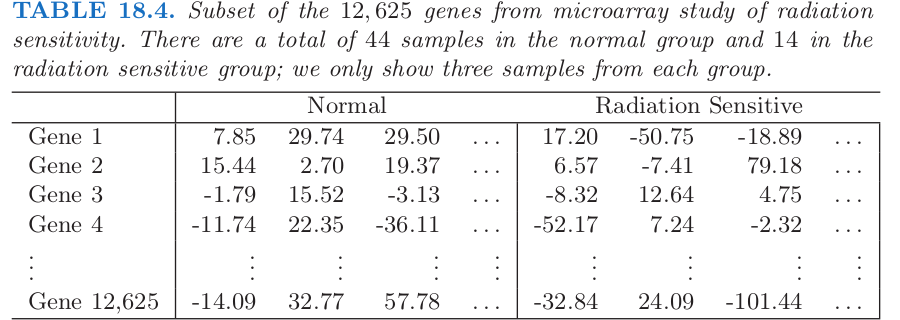
\includegraphics[width=\textwidth]{table18_4}
}

\frame{\frametitle{Feature Assessment when $p\gg N$: }
\framesubtitle{multiple testing problem}
The simplest way to identify significative genes:
\begin{itemize}
\item \textcolor{uio}{two-sample t-statistic} for each gene,
$$
t_j = \frac{\bar{x}_{2j} - \bar{x}_{1j}}{se_j}
$$
where
\begin{itemize}
\setlength\itemsep{5pt}
\item $\bar{x}_{kj} = \sum_{i\in C_k} x_{kj}/N_k$;
\item $C_k$ are the indexes of the $N_k$ observations of group $k$;
\item $se_j = \hat{\sigma}_j \sqrt{\frac{1}{N_1} + \frac{1}{N_2}}$;
\item $\hat{\sigma}^2_j = \frac{1}{N_1 + N_2 - 2}\left(\sum_{i\in C_1} (x_{ij} - \bar{x}_{1j})^2 + \sum_{i\in C_2} (x_{ij} - \bar{x}_{2j})^2 \right)$.
\end{itemize}
\end{itemize}
}

\frame{\frametitle{Feature Assessment when $p\gg N$: }
\framesubtitle{multiple testing problem}
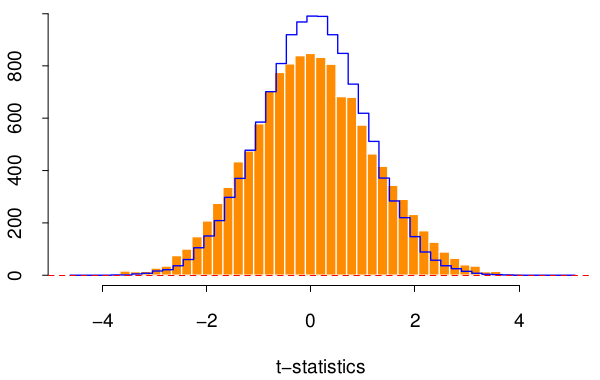
\includegraphics[width=\textwidth]{fig18_18}
}

\frame{\frametitle{Feature Assessment when $p\gg N$: }
\framesubtitle{multiple testing problem}
From the histogram ($12625$ t-statistics):
\begin{itemize}
 \item the values range \textcolor{uio}{from $-4.7$ to $5.0$};
 \item assuming $t_j \sim N(0,1)$, \textcolor{uio}{significance at $5\%$} when $|t_j| \geq 2$;
 \item in the example, \textcolor{uio}{$1189$ genes with $|t_j| \geq 2$}.
\end{itemize} 

\vspace{12pt}

However:
\begin{itemize}
 \item out of $12625$ genes, many are significant \textcolor{uio}{by chance};
 \item supposing (it is not true) independence:
 \begin{itemize}
 \item \textcolor{uio}{expected falsely significant} genes, $12625 \cdot 0.05 = \textcolor{uio}{631.25}$;
 \item standard deviation, $\sqrt{12625 \cdot 0.05 \cdot (1 - 0.05)} \approx 24.5$;
 \end{itemize}
 \item the actual 1189 is way \textcolor{uio}{out of range}.
\end{itemize} 
}

\frame{\frametitle{Feature Assessment when $p\gg N$: }
\framesubtitle{multiple testing problem}
Without assuming normality, \textcolor{uio}{permutation test}:
\begin{itemize}
\item perform $K =$ ${58}\choose{14}$ \textcolor{uio}{permutations of the sample labels};
\item compute the \textcolor{uio}{statistic $t_j^{[k]}$} for each permutation $k$;
\item the \textcolor{uio}{p-value for the gene $j$} is
$$
p_j = \frac{1}{K} \sum_{k = 1}^{K} \mathds{1}(|t_j^{[k]}| > |t_j|)
$$
\item[] (\textcolor{uio}{not all} ${58}\choose{14}$ are needed, \textcolor{uio}{random sample} of $K = 1000$)
\end{itemize}
}

\frame{\frametitle{Feature Assessment when $p\gg N$: }
\framesubtitle{multiple testing problem}
For $j \in 1,\dots,M$ test the hypotheses:
\begin{itemize}
\item[] H$_{0j}$: treatment has \textcolor{uio}{no effect} on gene $j$
\item[] H$_{1j}$: treatment \textcolor{uio}{has an effect} on gene $j$
\end{itemize}

\vspace{12pt}

H$_{0j}$ is \textcolor{uio}{rejected} at level $\alpha$ \textcolor{uio}{if $p_j < \alpha$}:
\begin{itemize}
\item $\alpha$ is the \textcolor{uio}{type-I error};
\item we expect a probability of \textcolor{uio}{falsely rejecting} H$_{0j}$ of $\alpha$.
\end{itemize}
}

\frame{\frametitle{Feature Assessment when $p\gg N$: }
\framesubtitle{family-wise error rate}
Define $A_j = \text{\{}H_{0j}$ is falsely rejected\} $\;\longrightarrow\;$ $Pr(A_j) = \alpha$.

\vspace{12pt}

The {\bf family-wise error rate} (FWER) is the probability of \textcolor{uio}{at least one} false rejection,
$$
Pr(A) = Pr(\bigcup_{j=1}^M A_j)
$$
\begin{itemize}
\item for $p$ large, \textcolor{uio}{$Pr(A) \gg \alpha$};
\item it depends on the \textcolor{uio}{correlation} between the test;
\item if tests independent, $Pr(A) = 1 - (1 - \alpha)^M$;
\item test with positive dependence, $Pr(A) \;\textcolor{uio}{<}\; 1 - (1 - \alpha)^M$;
\begin{itemize}
\item positive dependence is typical in genomic studies.
\end{itemize}
\end{itemize}
}


\frame{\frametitle{Feature Assessment when $p\gg N$: }
\framesubtitle{family-wise error rate}
The simplest approach to \textcolor{uio}{correct the p-value for the multiplicity} of the tests is the {\bf Bonferroni method}:
\begin{itemize}
\item reject $H_{0j}$ if \textcolor{uio}{$p_j < \alpha/M$};
\item it makes the individual test more stringent;
\item \textcolor{uio}{controls the FWER}
\begin{itemize}
\item it is easy to show that \textcolor{uio}{FWER $\leq \alpha$};
\end{itemize}
\item it is very (too) \textcolor{uio}{conservative}.
\end{itemize}

\vspace{12pt}

In the example:
\begin{itemize}
\item with $\alpha = 0.05$, $\alpha/M = 0.05/12635 \approx 3.9 \times 10^{-6}$;
\item \textcolor{uio}{no gene} has a p-value so small.
\end{itemize}
}


\subsection{The false discovery rate}

\frame{\frametitle{Feature Assessment when $p\gg N$: }
\framesubtitle{the false discovery rate}
Instead of FWER, we can control the {\bf false discovery rate} (FDR):
\begin{itemize}
\item \textcolor{uio}{expected proportion} of genes \textcolor{uio}{incorrectly defined significant among} those selected as \textcolor{uio}{significant},
\end{itemize}
\begin{center}
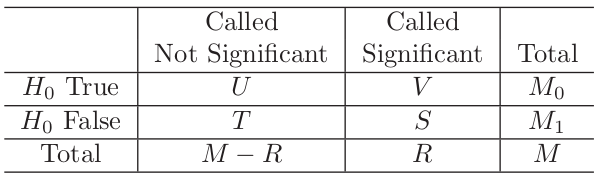
\includegraphics[width=0.75\textwidth]{table18_5}
\end{center}
\begin{itemize}
\item in formula, $\text{FDR} = E[V/R]$;
\item procedure to have the FDR \textcolor{uio}{smaller than an user-defined $\alpha$}.
\end{itemize}
}

\frame{\frametitle{Feature Assessment when $p\gg N$: }
\framesubtitle{the false discovery rate}
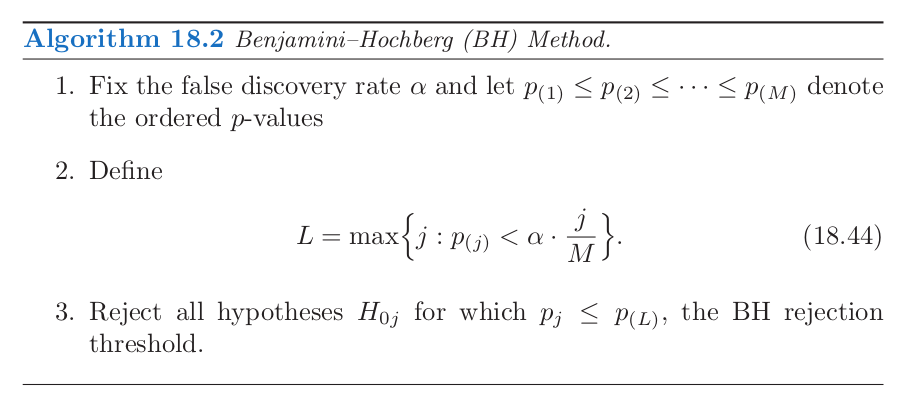
\includegraphics[width=\textwidth]{alg18_2}
}

\frame{\frametitle{Feature Assessment when $p\gg N$: }
\framesubtitle{the false discovery rate}
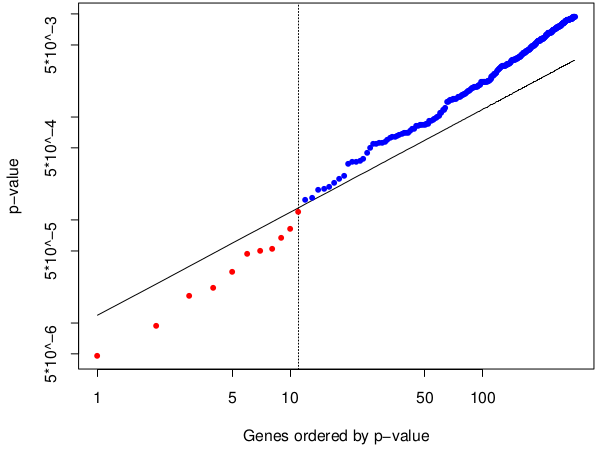
\includegraphics[width=\textwidth]{fig18_19}
}

\frame{\frametitle{Feature Assessment when $p\gg N$: }
\framesubtitle{the false discovery rate}
In the example:
\begin{itemize}
\item $\alpha = 0.15$;
\item the last $p_j$ \textcolor{uio}{under the line $\alpha \cdot (j/M)$} occurs at \textcolor{uio}{$j=11$};
\item the smallest 11 p-values are considered significative;
\item in the example, $p_{(11)} =  0.00012$;
\item the corresponding t-statistic is $|t_{(11)}| = 4.101$;
\item a gene is \textcolor{uio}{relevant} if the corresponding t-statistics is in absolute value larger than $4.101$.
\end{itemize}
}

\frame{\frametitle{Feature Assessment when $p\gg N$: }
\framesubtitle{the false discovery rate}
It can be proved \citep{BenjaminiHochberg1995} that
$$
\textcolor{uio}{\text{FDR} \leq \frac{M_0}{M}\alpha \leq \alpha}
$$
\begin{itemize}
\item \textcolor{uio}{regardless} the number of true null hypotheses;
\item \textcolor{uio}{regardless} the distribution of the p-values under $H_1$;
\item suppose \textcolor{uio}{independent test statistics};
\item in case of dependence, see \cite{BenjaminiYekutieli2001}.
\end{itemize}
}



\section{Stability Selection}

\subsection{Introduction}

\frame{\frametitle{Stability Selection: }
\framesubtitle{introduction}
In general:
\begin{itemize}
\item the \textcolor{uio}{$L_1$-penalty} is often use to perform model selection;
\item \textcolor{uio}{no oracle property} (strict conditions to have it);
\item issues with selecting the \textcolor{uio}{proper amount of regularization};
\end{itemize}

\vspace{12pt}

\cite{MeinshausenBuehlmann2010} suggested a procedure:
\begin{itemize}
\item based on \textcolor{uio}{subsampling} (could work with bootstrapping as well);
\item determines the \textcolor{uio}{amount of regularization to control the FWER};
\item \textcolor{uio}{new structure estimation} or variable selection scheme;
\item here presented with $L_1$-penalty, works in general.
\end{itemize}
}

\frame{\frametitle{Stability Selection: }
\framesubtitle{introduction}
Setting:
\begin{itemize}
\item $\beta$ is a $p$-dimensional vector of coefficients;
\item $S = \{j : \beta_j \neq 0\}$, \textcolor{uio}{$|S| < p$};
\item ${S}^C = \{j : \beta_j = 0\}$;
\item $Z^{[i]} = (X^{[i]}, Y^{[i]})$, $i = 1, \dots, N$, are the i.i.d.\ data,
\begin{itemize}
\item univariate response $Y$;
\item $N \times p$ covariate matrix $X$.
\end{itemize}
\item consider a \textcolor{uio}{linear model}
$$
Y = X\beta +\epsilon
$$
with $\epsilon = (\epsilon_1, \dots, \epsilon_N)$ with i.i.d.\ components.
\end{itemize}
}


\frame{\frametitle{Stability Selection: }
\framesubtitle{introduction}
The goal is to \textcolor{uio}{infer $S$ from the data}. We saw that lasso,
$$
\hat{\beta}^\lambda = \text{argmin}_{\beta \in \mathds{R}^p} \left(||Y - X\beta||_2^2 + \lambda \sum_{j = 1}^p |\beta_j|\right)
$$
provides an estimate of S, $S^\lambda = \{\textcolor{uio}{j: \hat{\beta}_j \neq 0}\} \subseteq \{1,\dots,p\}$.

\vspace{12pt}

Remember:
\begin{itemize}
\item \textcolor{uio}{$\lambda \in \mathds{R}^+$} is the regularization factor;
\item $||X_j||_2^2 = \sum_{i = 1}^N (x_j^{[i]})^2 = 1$;
\end{itemize}
}


\subsection{Selection probability}

\frame{\frametitle{Stability Selection: }
\framesubtitle{selection probability}
\textcolor{uio}{Stability selection} is \textcolor{uio}{built on} the concept of {\bf selection probability},

\vspace{6pt}

{\it Definition 1: Let $I$ be a random subsample of $\{1,\dots,N\}$ of size $\lfloor N/2 \rfloor$ drawn without replacement. We define \uline{selection probability} the probability for a variable $X_j$ of being in $S^\lambda(I)$,}
$$
\hat{\Pi}_j^\lambda = Pr^*[j \subseteq S^\lambda(I)]
$$

\vspace{6pt}

Note:
\begin{itemize}
\item $Pr^*$ is with respect of both the \textcolor{uio}{random subsampling} and \textcolor{uio}{other sources of randomness} if $S^\lambda$ is not deterministic;
\item $\lfloor N/2 \rfloor$ is chosen for \textcolor{uio}{computational efficiency}.
\end{itemize}
}


\subsection{Stability path}

\frame{\frametitle{Stability Selection: }
\framesubtitle{stability path}
Once we have the \textcolor{uio}{selection probability}, we can define the {\bf stability path}, as the \textcolor{uio}{evolution of $\hat{\Pi}_j^\lambda$} when $\lambda \in \Lambda$ varies,
\begin{itemize}
\item similar to the \textcolor{uio}{learning path plot} of lasso;
\item it shows the \textcolor{uio}{selection probabilities} for all variables;
\item it is very useful for \textcolor{uio}{improved} variable selection, especially in high-dimensional cases. 
\end{itemize}
}

\frame{\frametitle{Stability Selection: }
\framesubtitle{stability path}
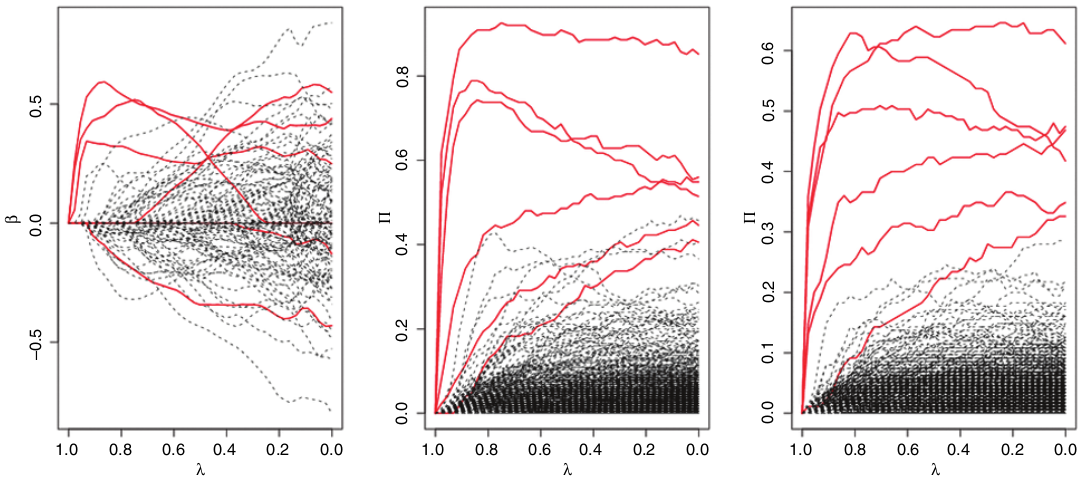
\includegraphics[width=\textwidth]{fig1_mb}
\footnotesize
\begin{itemize}
\item left: lasso learning path;
\item center: stability path of the lasso;
\item right: stability path of the randomized lasso.
\end{itemize}
}

\frame{\frametitle{Stability Selection: }
\framesubtitle{stability path}
Normally we would choose a \textcolor{uio}{specific $\lambda$}:
\begin{itemize}
\item it is a \textcolor{uio}{single element} of the set $\hat{S}^\lambda, \lambda \in \Lambda$;
\item $S$ might \textcolor{uio}{not} be a member of the set;
\item even if it is, it is \textcolor{uio}{hard to find} the right $\lambda$ high-dimensions.
\end{itemize}

\vspace{12pt}

With {\bf stability selection}:
\begin{itemize}
\item we do \textcolor{uio}{not} simply select one model in $\hat{S}^\lambda, \lambda \in \Lambda$;
\item the data are \textcolor{uio}{perturbed} (e.g. by subsampling) many times;
\item we choose all variables that occur in a \textcolor{uio}{large fraction} of the resulting selection sets.
\end{itemize}
}

\frame{\frametitle{Stability Selection: }
\framesubtitle{stability selection}
{\it Definition 2: For a cut-off $\pi_\text{thr}$, with $0 < \pi_\text{thr} < 1$, and a set of regularization parameters $\Lambda$, the \uline{set of stable variables} is defined as}
$$
\hat{S}^\text{stable} = \left\{j : \max_{\lambda\in\Lambda}(\Pi^\lambda_j) \geq \pi_\text{thr}\right\}.
$$
In this way:
\begin{itemize}
\item we \textcolor{uio}{keep variables} with a \textcolor{uio}{high selection} probability;
\item we \textcolor{uio}{disregard} those with \textcolor{uio}{low selection} probabilities;
\item the exact cut-off \textcolor{uio}{$\pi_\text{thr}$} is a \textcolor{uio}{tuning parameter};
\item the results vary surprisingly \textcolor{uio}{little} for sensible choices of $\pi_\text{thr}$;
\item results \textcolor{uio}{do not strongly depend} on the choice of $\lambda$ or $\Lambda$.
\end{itemize}
}


\subsection{Choice of regularization}

\frame{\frametitle{Stability Selection: }
\framesubtitle{choice of regularization}
Let:
\begin{itemize}
\item $S^\Lambda = \bigcup_{\lambda \in \Lambda} \hat{S}^\lambda$ be the \textcolor{uio}{set of selected variables} $\forall \lambda \in \Lambda$;
\item $q_\Lambda = E[|\hat{S}^\Lambda(I)|]$ be the \textcolor{uio}{average number} of selected variables;
\item $V = |S^C \bigcap \hat{S}^\text{stable}|$ the \textcolor{uio}{number of falsely selected} variables with stability selection.
\end{itemize}

\vspace{12pt}

{\it {\bf Theorem \citep{MeinshausenBuehlmann2010}}: Assuming that the distribution of $\{\mathds{1}_{j\in\hat{S}^\lambda}\}$ is exchangeable $\forall \lambda \in \Lambda$ and the procedure is not worse than a random guess, then}
$$
E[V] \leq \frac{1}{2\pi_\text{thr} - 1} \frac{q_\Lambda^2}{p}
$$
}

\frame{\frametitle{Stability Selection: }
\framesubtitle{choice of regularization}
Therefore:
\begin{itemize}
\setlength\itemsep{5pt}
\item $\pi_\text{thr}$ is a tuning parameter whose influence is very small;
\begin{itemize}
\item \textcolor{uio}{sensible values} are in $(0.6, 0.9)$;
\end{itemize}
\item once decided $\pi_\text{thr}$, $\Lambda$ is determined by the \textcolor{uio}{error control desired};
\item \textcolor{uio}{specifically} for $\pi_\text{thr} = 0.9$,
\begin{itemize}
\setlength\itemsep{2pt}
\item $\Lambda: q_\Lambda = \sqrt{0.8p} \quad \longrightarrow \quad E[V] \leq 1$;
\item $\Lambda: q_\Lambda = \sqrt{0.8\alpha p} \quad \longrightarrow \quad Pr[V>0] \leq \alpha$;
\end{itemize}
\item i.e., we need to find $\Lambda$ that gives a specific $q_\Lambda$,
\begin{itemize}
\setlength\itemsep{2pt}
\item $q$ is given by the \textcolor{uio}{number of variables} which enter in the model;
\item for lasso, find $\lambda_\text{min}: |\bigcup_{\lambda_\text{max} \geq \lambda \geq \lambda_\text{min}} \hat{S}^\lambda| \leq q$
\end{itemize}
\end{itemize}
}


\frame{\frametitle{Stability Selection: }
\framesubtitle{choice of regularization}
Final remarks:
\begin{itemize}
\item without stability selection, $\lambda$ depends on the \textcolor{uio}{unknown noise level of the observations};
\item the \textcolor{uio}{advantages} of stability selection are:
\begin{itemize}
\item \textcolor{uio}{exact error control} is possible;
\item the method works fine \textcolor{uio}{even though} the noise level is unknown;
\end{itemize}
\item real \textcolor{uio}{advantage} when $p \geq N$ (hard to estimate the noise level);
\item[]
\item \textcolor{uio}{consistency} can be proved \citep[see][for the proof for randomized lasso]{MeinshausenBuehlmann2010};
\item exchangeability in Theorem 1 is only need for the proof.
\end{itemize}
}


%%%%%%%%%%%
\section*{Bibliography}
%%%%%%%%%%%

\frame[allowframebreaks]{\frametitle{References}
\footnotesize
\bibliographystyle{../../../../support/biometrika}
\bibliography{../../../../support/biblio}
}

\end{document}
